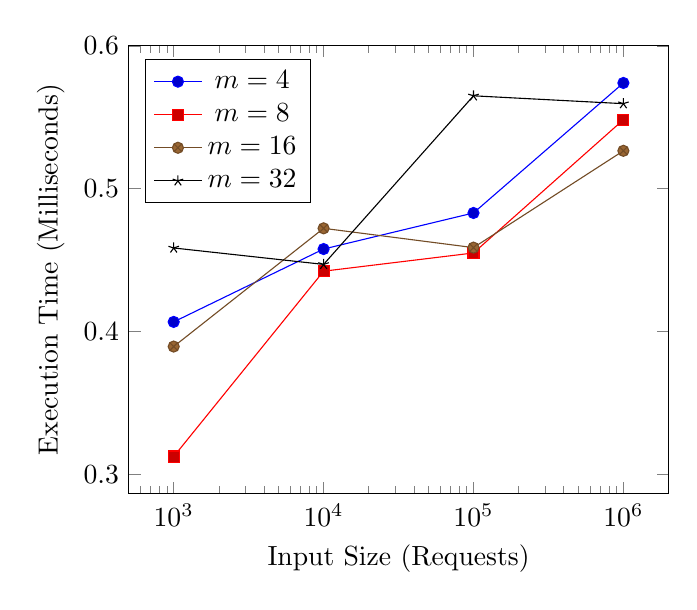
\begin{tikzpicture}
	\begin{axis}
		[
			xlabel={Input Size (Requests)},
			ylabel={Execution Time (Milliseconds)},
			legend pos=north west,
			domain=1:1000000,
			xmode=log,
		]
		\addplot+[cycle list name=color list]
			coordinates {
				(1000, 0.40675)
				(10000, 0.45775)
				(100000, 0.483)
				(1000000, 0.574)
			};
		\addlegendentry{$m=4$}
		\addplot+[cycle list name=color list]
			coordinates {
				(1000, 0.3125)
				(10000, 0.44225)
				(100000, 0.455)
				(1000000, 0.54825)
			};
		\addlegendentry{$m=8$}
		\addplot+[cycle list name=color list]
			coordinates {
				(1000, 0.3895)
				(10000, 0.47225)
				(100000, 0.45875)
				(1000000, 0.5265)
			};
		\addlegendentry{$m=16$}
		\addplot+[cycle list name=color list]
			coordinates {
				(1000, 0.4585)
				(10000, 0.447)
				(100000, 0.565)
				(1000000, 0.5595)
			};
		\addlegendentry{$m=32$}
	\end{axis}
\end{tikzpicture}
